%---------------------------------------------
%
%       START
%
%---------------------------------------------

\chapter{Supplementary data to \Chapref{missing_mammals}}
%\chapter{Supplementary Information to \Chapref{Longevity}}%labstudy is the label for chapter 2.
\label{chap:Appendix_missing_mammals}

\bigskip
\medskip
\begin{center}

\noindent{\Large \bf Assessment of cladistic data availability for living mammals} \\
bigskip
\end{center}
%---------------------------------------------
%
%       ABSTRACT
%
%---------------------------------------------
The following section contains supplementary results to the chapter ``Assessment of cladistic data availability for living mammals'': the available data structure using the NTI and the PD metric; the proportion of available data and the data structure for all the matrices (including the matrices with less than 100 characters); and phylogenetical representation of the data availability per order (excluding Primates and Carnivora, present in the main body).

% latex table generated in R 3.2.0 by xtable 1.7-4 package
% Sat Jun 20 17:19:07 2015
\begin{longtable}{lL{1.8cm}C{2cm}ccc}
\caption[Number of taxa with available cladistic data for mammalian orders without any character threshold]{\textbf{Number of taxa with available cladistic data for mammalian orders at three taxonomic levels (without any character threshold; results from the 286 matrices).} The coverage represents the proportion of taxa with available morphological data. The left vertical bar represents 25\% of available data (``low'' coverage if \textless 25\%); The right vertical bar represents 75\% of available data (``high'' coverage if \textgreater 75\%). When the Net Relatedness Index (NRI) and the Nearest Taxon Index (NTI) are negative, taxa are more phylogenetically dispersed than expected by chance; when NRI or NTI are positive, taxa are more phylogenetically clustered by expected by chance. Significant NRI or NTI are highlighted in bold. *p \textless 0.05; **p \textless 0.01; ***p \textless 0.001.} \\ 
  \hline
\textbf{Order} & \textbf{Taxonomic level} & \textbf{Proportion of taxa} & \textbf{Coverage} & \textbf{NRI} & \textbf{NTI} \\ 
  \hline
Afrosoricida & family & 2/2 & 
\includegraphics[width=0.20\linewidth, height=0.05\linewidth]{Supplementaries/Figures/MissingMammals/Results_1c/Table_figures/bar1.pdf} &   &   \\ 
  Afrosoricida & genus & 17/17 & 
\includegraphics[width=0.20\linewidth, height=0.05\linewidth]{Supplementaries/Figures/MissingMammals/Results_1c/Table_figures/bar2.pdf} &   &   \\ 
  Afrosoricida & species & 23/42 & 
\includegraphics[width=0.20\linewidth, height=0.05\linewidth]{Supplementaries/Figures/MissingMammals/Results_1c/Table_figures/bar3.pdf} & 1.75 & 1.08 \\ 
  Carnivora & family & 14/15 & 
\includegraphics[width=0.20\linewidth, height=0.05\linewidth]{Supplementaries/Figures/MissingMammals/Results_1c/Table_figures/bar4.pdf} & 0.63 & 0.6 \\ 
  \textbf{Carnivora} & \textbf{genus} & \textbf{54/125} & 
\includegraphics[width=0.20\linewidth, height=0.05\linewidth]{Supplementaries/Figures/MissingMammals/Results_1c/Table_figures/bar5.pdf} & \textbf{4.81**} & \textbf{1.78*} \\ 
  \textbf{Carnivora} & \textbf{species} & \textbf{76/283} & 
\includegraphics[width=0.20\linewidth, height=0.05\linewidth]{Supplementaries/Figures/MissingMammals/Results_1c/Table_figures/bar6.pdf} & \textbf{7.66**} & \textbf{0.85} \\ 
  Cetartiodactyla & family & 21/21 & 
\includegraphics[width=0.20\linewidth, height=0.05\linewidth]{Supplementaries/Figures/MissingMammals/Results_1c/Table_figures/bar7.pdf} &   &   \\ 
  Cetartiodactyla & genus & 100/128 & 
\includegraphics[width=0.20\linewidth, height=0.05\linewidth]{Supplementaries/Figures/MissingMammals/Results_1c/Table_figures/bar8.pdf} & 0.85 & 0.94 \\ 
  \textbf{Cetartiodactyla} & \textbf{species} & \textbf{171/310} & 
\includegraphics[width=0.20\linewidth, height=0.05\linewidth]{Supplementaries/Figures/MissingMammals/Results_1c/Table_figures/bar9.pdf} & \textbf{1.92*} & \textbf{-0.46} \\ 
  Chiroptera & family & 15/18 & 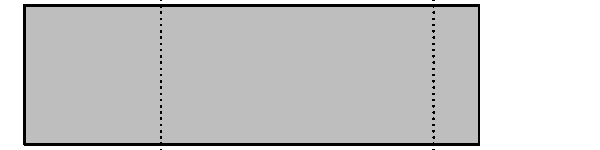
\includegraphics[width=0.20\linewidth, height=0.05\linewidth]{Supplementaries/Figures/MissingMammals/Results_1c/Table_figures/bar10.pdf} & -0.28 & 0.56 \\ 
  \textbf{Chiroptera} & \textbf{genus} & \textbf{93/202} & 
\includegraphics[width=0.20\linewidth, height=0.05\linewidth]{Supplementaries/Figures/MissingMammals/Results_1c/Table_figures/bar11.pdf} & \textbf{13.47**} & \textbf{1.1} \\ 
  \textbf{Chiroptera} & \textbf{species} & \textbf{215/1053} & 
\includegraphics[width=0.20\linewidth, height=0.05\linewidth]{Supplementaries/Figures/MissingMammals/Results_1c/Table_figures/bar12.pdf} & \textbf{8.82**} & \textbf{1.22} \\ 
  Cingulata & family & 1/1 & 
\includegraphics[width=0.20\linewidth, height=0.05\linewidth]{Supplementaries/Figures/MissingMammals/Results_1c/Table_figures/bar13.pdf} &   &   \\ 
  Cingulata & genus & 8/9 & 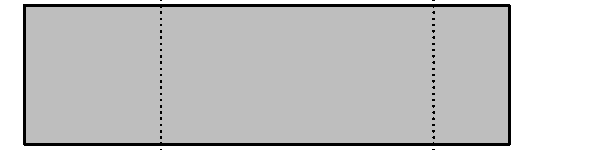
\includegraphics[width=0.20\linewidth, height=0.05\linewidth]{Supplementaries/Figures/MissingMammals/Results_1c/Table_figures/bar14.pdf} & 1.51 & -1.57 \\ 
  \textbf{Cingulata} & \textbf{species} & \textbf{9/29} & 
\includegraphics[width=0.20\linewidth, height=0.05\linewidth]{Supplementaries/Figures/MissingMammals/Results_1c/Table_figures/bar15.pdf} & \textbf{1.9*} & \textbf{0.11} \\ 
  Dasyuromorphia & family & 2/2 & 
\includegraphics[width=0.20\linewidth, height=0.05\linewidth]{Supplementaries/Figures/MissingMammals/Results_1c/Table_figures/bar16.pdf} &   &   \\ 
  Dasyuromorphia & genus & 8/22 & 
\includegraphics[width=0.20\linewidth, height=0.05\linewidth]{Supplementaries/Figures/MissingMammals/Results_1c/Table_figures/bar17.pdf} & -0.75 & -1.07 \\ 
  Dasyuromorphia & species & 9/64 & 
\includegraphics[width=0.20\linewidth, height=0.05\linewidth]{Supplementaries/Figures/MissingMammals/Results_1c/Table_figures/bar18.pdf} & -0.88 & -0.34 \\ 
  Dermoptera & family & 1/1 & 
\includegraphics[width=0.20\linewidth, height=0.05\linewidth]{Supplementaries/Figures/MissingMammals/Results_1c/Table_figures/bar19.pdf} &   &   \\ 
  Dermoptera & genus & 1/2 & 
\includegraphics[width=0.20\linewidth, height=0.05\linewidth]{Supplementaries/Figures/MissingMammals/Results_1c/Table_figures/bar20.pdf} &   &   \\ 
  Dermoptera & species & 1/2 & 
\includegraphics[width=0.20\linewidth, height=0.05\linewidth]{Supplementaries/Figures/MissingMammals/Results_1c/Table_figures/bar21.pdf} &   &   \\ 
  Didelphimorphia & family & 1/1 & 
\includegraphics[width=0.20\linewidth, height=0.05\linewidth]{Supplementaries/Figures/MissingMammals/Results_1c/Table_figures/bar22.pdf} &   &   \\ 
  Didelphimorphia & genus & 16/16 & 
\includegraphics[width=0.20\linewidth, height=0.05\linewidth]{Supplementaries/Figures/MissingMammals/Results_1c/Table_figures/bar23.pdf} &   &   \\ 
  Didelphimorphia & species & 42/84 & 
\includegraphics[width=0.20\linewidth, height=0.05\linewidth]{Supplementaries/Figures/MissingMammals/Results_1c/Table_figures/bar24.pdf} & -1.65 & 0.2 \\ 
  Diprotodontia & family & 11/11 & 
\includegraphics[width=0.20\linewidth, height=0.05\linewidth]{Supplementaries/Figures/MissingMammals/Results_1c/Table_figures/bar25.pdf} &   &   \\ 
  Diprotodontia & genus & 25/38 & 
\includegraphics[width=0.20\linewidth, height=0.05\linewidth]{Supplementaries/Figures/MissingMammals/Results_1c/Table_figures/bar26.pdf} & -1.13 & -1.31 \\ 
  Diprotodontia & species & 31/126 & 
\includegraphics[width=0.20\linewidth, height=0.05\linewidth]{Supplementaries/Figures/MissingMammals/Results_1c/Table_figures/bar27.pdf} & 0.48 & -1.77 \\ 
  Erinaceomorpha & family & 1/1 & 
\includegraphics[width=0.20\linewidth, height=0.05\linewidth]{Supplementaries/Figures/MissingMammals/Results_1c/Table_figures/bar28.pdf} &   &   \\ 
  Erinaceomorpha & genus & 10/10 & 
\includegraphics[width=0.20\linewidth, height=0.05\linewidth]{Supplementaries/Figures/MissingMammals/Results_1c/Table_figures/bar29.pdf} &   &   \\ 
  Erinaceomorpha & species & 21/22 & 
\includegraphics[width=0.20\linewidth, height=0.05\linewidth]{Supplementaries/Figures/MissingMammals/Results_1c/Table_figures/bar30.pdf} & -1.07 & -0.2 \\ 
  Hyracoidea & family & 1/1 & 
\includegraphics[width=0.20\linewidth, height=0.05\linewidth]{Supplementaries/Figures/MissingMammals/Results_1c/Table_figures/bar31.pdf} &   &   \\ 
  Hyracoidea & genus & 1/3 & 
\includegraphics[width=0.20\linewidth, height=0.05\linewidth]{Supplementaries/Figures/MissingMammals/Results_1c/Table_figures/bar32.pdf} &   &   \\ 
  Hyracoidea & species & 1/4 & 
\includegraphics[width=0.20\linewidth, height=0.05\linewidth]{Supplementaries/Figures/MissingMammals/Results_1c/Table_figures/bar33.pdf} &   &   \\ 
  Lagomorpha & family & 2/2 & 
\includegraphics[width=0.20\linewidth, height=0.05\linewidth]{Supplementaries/Figures/MissingMammals/Results_1c/Table_figures/bar34.pdf} &   &   \\ 
  Lagomorpha & genus & 5/12 & 
\includegraphics[width=0.20\linewidth, height=0.05\linewidth]{Supplementaries/Figures/MissingMammals/Results_1c/Table_figures/bar35.pdf} & -1.06 & -0.95 \\ 
  Lagomorpha & species & 12/86 & 
\includegraphics[width=0.20\linewidth, height=0.05\linewidth]{Supplementaries/Figures/MissingMammals/Results_1c/Table_figures/bar36.pdf} & -0.62 & -1.88 \\ 
  Macroscelidea & family & 1/1 & 
\includegraphics[width=0.20\linewidth, height=0.05\linewidth]{Supplementaries/Figures/MissingMammals/Results_1c/Table_figures/bar37.pdf} &   &   \\ 
  Macroscelidea & genus & 4/4 & 
\includegraphics[width=0.20\linewidth, height=0.05\linewidth]{Supplementaries/Figures/MissingMammals/Results_1c/Table_figures/bar38.pdf} &   &   \\ 
  Macroscelidea & species & 12/15 & 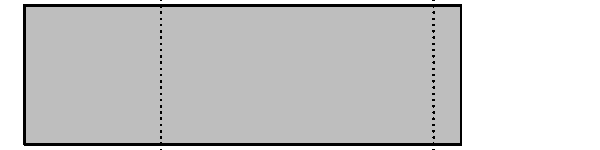
\includegraphics[width=0.20\linewidth, height=0.05\linewidth]{Supplementaries/Figures/MissingMammals/Results_1c/Table_figures/bar39.pdf} & -1.3 & -1.06 \\ 
  Microbiotheria & family & 1/1 & 
\includegraphics[width=0.20\linewidth, height=0.05\linewidth]{Supplementaries/Figures/MissingMammals/Results_1c/Table_figures/bar40.pdf} &   &   \\ 
  Microbiotheria & genus & 1/1 & 
\includegraphics[width=0.20\linewidth, height=0.05\linewidth]{Supplementaries/Figures/MissingMammals/Results_1c/Table_figures/bar41.pdf} &   &   \\ 
  Microbiotheria & species & 1/1 & 
\includegraphics[width=0.20\linewidth, height=0.05\linewidth]{Supplementaries/Figures/MissingMammals/Results_1c/Table_figures/bar42.pdf} &   &   \\ 
  Monotremata & family & 2/2 & 
\includegraphics[width=0.20\linewidth, height=0.05\linewidth]{Supplementaries/Figures/MissingMammals/Results_1c/Table_figures/bar43.pdf} &   &   \\ 
  Monotremata & genus & 2/3 & 
\includegraphics[width=0.20\linewidth, height=0.05\linewidth]{Supplementaries/Figures/MissingMammals/Results_1c/Table_figures/bar44.pdf} & -0.72 & -0.69 \\ 
  Monotremata & species & 2/4 & 
\includegraphics[width=0.20\linewidth, height=0.05\linewidth]{Supplementaries/Figures/MissingMammals/Results_1c/Table_figures/bar45.pdf} & -0.97 & -0.97 \\ 
  Notoryctemorphia & family & 1/1 & 
\includegraphics[width=0.20\linewidth, height=0.05\linewidth]{Supplementaries/Figures/MissingMammals/Results_1c/Table_figures/bar46.pdf} &   &   \\ 
  Notoryctemorphia & genus & 1/1 & 
\includegraphics[width=0.20\linewidth, height=0.05\linewidth]{Supplementaries/Figures/MissingMammals/Results_1c/Table_figures/bar47.pdf} &   &   \\ 
  Notoryctemorphia & species & 0/2 & 
\includegraphics[width=0.20\linewidth, height=0.05\linewidth]{Supplementaries/Figures/MissingMammals/Results_1c/Table_figures/bar48.pdf} &   &   \\ 
  Paucituberculata & family & 1/1 & 
\includegraphics[width=0.20\linewidth, height=0.05\linewidth]{Supplementaries/Figures/MissingMammals/Results_1c/Table_figures/bar49.pdf} &   &   \\ 
  Paucituberculata & genus & 3/3 & 
\includegraphics[width=0.20\linewidth, height=0.05\linewidth]{Supplementaries/Figures/MissingMammals/Results_1c/Table_figures/bar50.pdf} &   &   \\ 
  Paucituberculata & species & 5/5 & \includegraphics[width=0.20\linewidth, height=0.05\linewidth]{Supplementaries/Figures/MissingMammals/Results_1c/Table_figures/bar51.pdf} &   &   \\ 
  Peramelemorphia & family & 2/2 & \includegraphics[width=0.20\linewidth, height=0.05\linewidth]{Supplementaries/Figures/MissingMammals/Results_1c/Table_figures/bar52.pdf} &   &   \\ 
  Peramelemorphia & genus & 7/7 & \includegraphics[width=0.20\linewidth, height=0.05\linewidth]{Supplementaries/Figures/MissingMammals/Results_1c/Table_figures/bar53.pdf} &   &   \\ 
  Peramelemorphia & species & 16/18 & \includegraphics[width=0.20\linewidth, height=0.05\linewidth]{Supplementaries/Figures/MissingMammals/Results_1c/Table_figures/bar54.pdf} & -0.13 & 0.97 \\ 
  Perissodactyla & family & 3/3 & \includegraphics[width=0.20\linewidth, height=0.05\linewidth]{Supplementaries/Figures/MissingMammals/Results_1c/Table_figures/bar55.pdf} &   &   \\ 
  Perissodactyla & genus & 6/6 & \includegraphics[width=0.20\linewidth, height=0.05\linewidth]{Supplementaries/Figures/MissingMammals/Results_1c/Table_figures/bar56.pdf} &   &   \\ 
  Perissodactyla & species & 10/16 & \includegraphics[width=0.20\linewidth, height=0.05\linewidth]{Supplementaries/Figures/MissingMammals/Results_1c/Table_figures/bar57.pdf} & -0.07 & -2.63 \\ 
  Pholidota & family & 1/1 & \includegraphics[width=0.20\linewidth, height=0.05\linewidth]{Supplementaries/Figures/MissingMammals/Results_1c/Table_figures/bar58.pdf} &   &   \\ 
  Pholidota & genus & 1/1 & \includegraphics[width=0.20\linewidth, height=0.05\linewidth]{Supplementaries/Figures/MissingMammals/Results_1c/Table_figures/bar59.pdf} &   &   \\ 
  Pholidota & species & 4/8 & \includegraphics[width=0.20\linewidth, height=0.05\linewidth]{Supplementaries/Figures/MissingMammals/Results_1c/Table_figures/bar60.pdf} & 1.18 & 0.94 \\ 
  Pilosa & family & 4/5 & \includegraphics[width=0.20\linewidth, height=0.05\linewidth]{Supplementaries/Figures/MissingMammals/Results_1c/Table_figures/bar61.pdf} & 1.87 & 2 \\ 
  Pilosa & genus & 4/5 & \includegraphics[width=0.20\linewidth, height=0.05\linewidth]{Supplementaries/Figures/MissingMammals/Results_1c/Table_figures/bar62.pdf} & -0.96 & 0.36 \\ 
  \textbf{Pilosa} & \textbf{species} & \textbf{5/29} & \includegraphics[width=0.20\linewidth, height=0.05\linewidth]{Supplementaries/Figures/MissingMammals/Results_1c/Table_figures/bar63.pdf} & \textbf{1.28} & \textbf{2.38*} \\ 
  Primates & family & 15/15 & \includegraphics[width=0.20\linewidth, height=0.05\linewidth]{Supplementaries/Figures/MissingMammals/Results_1c/Table_figures/bar64.pdf} &   &   \\ 
  Primates & genus & 48/68 & \includegraphics[width=0.20\linewidth, height=0.05\linewidth]{Supplementaries/Figures/MissingMammals/Results_1c/Table_figures/bar65.pdf} & -0.35 & -1.33 \\ 
  Primates & species & 64/351 & \includegraphics[width=0.20\linewidth, height=0.05\linewidth]{Supplementaries/Figures/MissingMammals/Results_1c/Table_figures/bar66.pdf} & -0.67 & -1.27 \\ 
  Proboscidea & family & 1/1 & \includegraphics[width=0.20\linewidth, height=0.05\linewidth]{Supplementaries/Figures/MissingMammals/Results_1c/Table_figures/bar67.pdf} &   &   \\ 
  Proboscidea & genus & 2/2 & \includegraphics[width=0.20\linewidth, height=0.05\linewidth]{Supplementaries/Figures/MissingMammals/Results_1c/Table_figures/bar68.pdf} &   &   \\ 
  Proboscidea & species & 2/3 & \includegraphics[width=0.20\linewidth, height=0.05\linewidth]{Supplementaries/Figures/MissingMammals/Results_1c/Table_figures/bar69.pdf} & -0.69 & -0.69 \\ 
  Rodentia & family & 18/32 & \includegraphics[width=0.20\linewidth, height=0.05\linewidth]{Supplementaries/Figures/MissingMammals/Results_1c/Table_figures/bar70.pdf} & 0.66 & -0.98 \\ 
  Rodentia & genus & 82/450 & \includegraphics[width=0.20\linewidth, height=0.05\linewidth]{Supplementaries/Figures/MissingMammals/Results_1c/Table_figures/bar71.pdf} & -1.66 & 1.55 \\ 
  \textbf{Rodentia} & \textbf{species} & \textbf{90/2094} & \includegraphics[width=0.20\linewidth, height=0.05\linewidth]{Supplementaries/Figures/MissingMammals/Results_1c/Table_figures/bar72.pdf} & \textbf{2.76*} & \textbf{2.34*} \\ 
  Scandentia & family & 2/2 & \includegraphics[width=0.20\linewidth, height=0.05\linewidth]{Supplementaries/Figures/MissingMammals/Results_1c/Table_figures/bar73.pdf} &   &   \\ 
  Scandentia & genus & 2/5 & \includegraphics[width=0.20\linewidth, height=0.05\linewidth]{Supplementaries/Figures/MissingMammals/Results_1c/Table_figures/bar74.pdf} & -0.74 & -0.74 \\ 
  Scandentia & species & 3/20 & \includegraphics[width=0.20\linewidth, height=0.05\linewidth]{Supplementaries/Figures/MissingMammals/Results_1c/Table_figures/bar75.pdf} & -1.88 & -0.84 \\ 
  Sirenia & family & 2/2 & \includegraphics[width=0.20\linewidth, height=0.05\linewidth]{Supplementaries/Figures/MissingMammals/Results_1c/Table_figures/bar76.pdf} &   &   \\ 
  Sirenia & genus & 2/2 & \includegraphics[width=0.20\linewidth, height=0.05\linewidth]{Supplementaries/Figures/MissingMammals/Results_1c/Table_figures/bar77.pdf} &   &   \\ 
  Sirenia & species & 4/4 & \includegraphics[width=0.20\linewidth, height=0.05\linewidth]{Supplementaries/Figures/MissingMammals/Results_1c/Table_figures/bar78.pdf} &   &   \\ 
  Soricomorpha & family & 3/4 & \includegraphics[width=0.20\linewidth, height=0.05\linewidth]{Supplementaries/Figures/MissingMammals/Results_1c/Table_figures/bar79.pdf} & -0.98 & -0.99 \\ 
  \textbf{Soricomorpha} & \textbf{genus} & \textbf{19/43} & \includegraphics[width=0.20\linewidth, height=0.05\linewidth]{Supplementaries/Figures/MissingMammals/Results_1c/Table_figures/bar80.pdf} & \textbf{7.11**} & \textbf{2.59**} \\ 
  \textbf{Soricomorpha} & \textbf{species} & \textbf{21/392} & \includegraphics[width=0.20\linewidth, height=0.05\linewidth]{Supplementaries/Figures/MissingMammals/Results_1c/Table_figures/bar81.pdf} & \textbf{10.65**} & \textbf{3.56**} \\ 
  Tubulidentata & family & 1/1 & \includegraphics[width=0.20\linewidth, height=0.05\linewidth]{Supplementaries/Figures/MissingMammals/Results_1c/Table_figures/bar82.pdf} &   &   \\ 
  Tubulidentata & genus & 1/1 & \includegraphics[width=0.20\linewidth, height=0.05\linewidth]{Supplementaries/Figures/MissingMammals/Results_1c/Table_figures/bar83.pdf} &   &   \\ 
  Tubulidentata & species & 1/1 & \includegraphics[width=0.20\linewidth, height=0.05\linewidth]{Supplementaries/Figures/MissingMammals/Results_1c/Table_figures/bar84.pdf} &   &   \\ 
   \hline
\hline
\label{MissingMammals_Supp_table}
\end{longtable}


\begin{figure}[!ht]
\centering
    \includegraphics[height=0.4\textheight]{Supplementaries/Figures/MissingMammals/Supp_figure_AFROSORICIDA.pdf}
\caption[Distribution of available morphological data across Afrosoricida]{Distribution of available morphological data across Afrosoricida. Edges are colored in grey when no morphological data is available or in blue when data is available.}
\label{Supp_Figure_Phylo-Afrosoricida}
\end{figure}

\begin{figure}[!ht]
\centering
    \includegraphics[height=0.4\textheight]{Supplementaries/Figures/MissingMammals/Supp_figure_CHIROPTERA.pdf}
\caption[Distribution of available morphological data across Chiroptera]{Distribution of available morphological data across Chiroptera. Edges are colored in grey when no morphological data is available or in blue when data is available.}
\label{Supp_Figure_Phylo-Chiroptera}
\end{figure}

\begin{figure}[!ht]
\centering
    \includegraphics[height=0.4\textheight]{Supplementaries/Figures/MissingMammals/Supp_figure_CINGULATA.pdf}
\caption[Distribution of available morphological data across Cingulata]{Distribution of available morphological data across Cingulata. Edges are colored in grey when no morphological data is available or in blue when data is available.}
\label{Supp_Figure_Phylo-Cingulata}
\end{figure}

\begin{figure}[!ht]
\centering
    \includegraphics[height=0.4\textheight]{Supplementaries/Figures/MissingMammals/Supp_figure_DASYUROMORPHIA.pdf}
\caption[Distribution of available morphological data across Dasyuromorphia]{Distribution of available morphological data across Dasyuromorphia. Edges are colored in grey when no morphological data is available or in blue when data is available.}
\label{Supp_Figure_Phylo-Dasyuromorphia}
\end{figure}

\begin{figure}[!ht]
\centering
    \includegraphics[height=0.4\textheight]{Supplementaries/Figures/MissingMammals/Supp_figure_DIDELPHIMORPHIA.pdf}
\caption[Distribution of available morphological data across Didelphimorphia]{Distribution of available morphological data across Didelphimorphia. Edges are colored in grey when no morphological data is available or in blue when data is available.}
\label{Supp_Figure_Phylo-Didelphimorphia}
\end{figure}

\begin{figure}[!ht]
\centering
    \includegraphics[height=0.4\textheight]{Supplementaries/Figures/MissingMammals/Supp_figure_DIPROTODONTIA.pdf}
\caption[Distribution of available morphological data across Diprotodontia]{Distribution of available morphological data across Diprotodontia. Edges are colored in grey when no morphological data is available or in blue when data is available.}
\label{Supp_Figure_Phylo-Diprotodontia}
\end{figure}

\begin{figure}[!ht]
\centering
    \includegraphics[height=0.4\textheight]{Supplementaries/Figures/MissingMammals/Supp_figure_ERINACEOMORPHA.pdf}
\caption[Distribution of available morphological data across Erinaceomorpha]{Distribution of available morphological data across Erinaceomorpha. Edges are colored in grey when no morphological data is available or in blue when data is available.}
\label{Supp_Figure_Phylo-Erinaceomorpha}
\end{figure}

\begin{figure}[!ht]
\centering
    \includegraphics[height=0.4\textheight]{Supplementaries/Figures/MissingMammals/Supp_figure_PILOSA.pdf}
\caption[Distribution of available morphological data across Pilosa]{Distribution of available morphological data across Pilosa. Edges are colored in grey when no morphological data is available or in blue when data is available.}
\label{Supp_Figure_Phylo-Pilosa}
\end{figure}

\begin{figure}[!ht]
\centering
    \includegraphics[height=0.4\textheight]{Supplementaries/Figures/MissingMammals/Supp_figure_CETARTIODACTYLA.pdf}
\caption[Distribution of available morphological data across Cetartiodactyla]{Distribution of available morphological data across Cetartiodactyla. Edges are colored in grey when no morphological data is available or in blue when data is available.}
\label{Supp_Figure_Phylo-Primates}
\end{figure}

\begin{figure}[!ht]
\centering
    \includegraphics[height=0.4\textheight]{Supplementaries/Figures/MissingMammals/Supp_figure_RODENTIA.pdf}
\caption[Distribution of available morphological data across Rodentia]{Distribution of available morphological data across Rodentia. Edges are colored in grey when no morphological data is available or in blue when data is available.}
\label{Supp_Figure_Phylo-Rodentia}
\end{figure}

\begin{figure}[!ht]
\centering
    \includegraphics[height=0.4\textheight]{Supplementaries/Figures/MissingMammals/Supp_figure_SCANDENTIA.pdf}
\caption[Distribution of available morphological data across Scandentia]{Distribution of available morphological data across Scandentia. Edges are colored in grey when no morphological data is available or in blue when data is available.}
\label{Supp_Figure_Phylo-Scandentia}
\end{figure}

\begin{figure}[!ht]
\centering
    \includegraphics[height=0.4\textheight]{Supplementaries/Figures/MissingMammals/Supp_figure_SORICOMORPHA.pdf}
\caption[Distribution of available morphological data across Soricomorpha]{Distribution of available morphological data across Soricomorpha. Edges are colored in grey when no morphological data is available or in blue when data is available.}
\label{Supp_Figure_Phylo-Soricomorpha}
\end{figure}
